\capitulo{3}{Conceptos teóricos}

%En aquellos proyectos que necesiten para su comprensión y desarrollo de unos conceptos teóricos de una determinada materia o de un determinado dominio de conocimiento, debe existir un apartado que sintetice dichos conceptos.
%
%Algunos conceptos teóricos de \LaTeX \footnote{Créditos a los proyectos de Álvaro López Cantero: Configurador de Presupuestos y Roberto Izquierdo Amo: PLQuiz}.
%
%\section{Secciones}
%
%Las secciones se incluyen con el comando section.
%
%\subsection{Subsecciones}
%
%Además de secciones tenemos subsecciones.
%
%\subsubsection{Subsubsecciones}
%
%Y subsecciones. 
%
%
%\section{Referencias}
%
%Las referencias se incluyen en el texto usando cite \cite{wiki:latex}. Para citar webs, artículos o libros \cite{koza92}.
%
%
%\section{Imágenes}
%
%Se pueden incluir imágenes con los comandos standard de \LaTeX, pero esta plantilla dispone de comandos propios como por ejemplo el siguiente:
%
%\imagen{escudoInfor}{Autómata para una expresión vacía}
%
%
%
%\section{Listas de items}
%
%Existen tres posibilidades:
%
%\begin{itemize}
%	\item primer item.
%	\item segundo item.
%\end{itemize}
%
%\begin{enumerate}
%	\item primer item.
%	\item segundo item.
%\end{enumerate}
%
%\begin{description}
%	\item[Primer item] más información sobre el primer item.
%	\item[Segundo item] más información sobre el segundo item.
%\end{description}
%	
%\begin{itemize}
%\item 
%\end{itemize}
%
%\section{Tablas}
%
%Igualmente se pueden usar los comandos específicos de \LaTeX o bien usar alguno de los comandos de la plantilla.
%
%\tablaSmall{Herramientas y tecnologías utilizadas en cada parte del proyecto}{l c c c c}{herramientasportipodeuso}
%{ \multicolumn{1}{l}{Herramientas} & App AngularJS & API REST & BD & Memoria \\}{ 
%HTML5 & X & & &\\
%CSS3 & X & & &\\
%BOOTSTRAP & X & & &\\
%JavaScript & X & & &\\
%AngularJS & X & & &\\
%Bower & X & & &\\
%PHP & & X & &\\
%Karma + Jasmine & X & & &\\
%Slim framework & & X & &\\
%Idiorm & & X & &\\
%Composer & & X & &\\
%JSON & X & X & &\\
%PhpStorm & X & X & &\\
%MySQL & & & X &\\
%PhpMyAdmin & & & X &\\
%Git + BitBucket & X & X & X & X\\
%Mik\TeX{} & & & & X\\
%\TeX{}Maker & & & & X\\
%Astah & & & & X\\
%Balsamiq Mockups & X & & &\\
%VersionOne & X & X & X & X\\
%}
En este capítulo se explican conceptos relevantes para la comprensión de este proyecto y su contexto.
\section{Calidad de proceso y producto software}
Todo proyecto de software tienen como objetivo desarrollar software de alta calidad, que cumpla con los requisitos acordados. Sin embargo, la calidad de un producto de software no tiene que ver solo con que se cumplan todos los requisitos funcionales, sino también otros requerimientos no funcionales que no se incluyen en la especificación como los de mantenimiento.

%Comentar fig 25.3 - Ppales factores de la calidad de protducto software p561
Sommerville enumera en \textit{Software Engineering} \cite{sommerville_ingenierisoftware_2002} los principales factores que afectan a la calidad del producto, como se puede observar en la figura \ref{fig:M3-FactoresCalidad}:
\begin{itemize}
	\tightlist
	\item Calidad del proceso
	\item Tecnología de desarrollo
	\item Calidad del personal
	\item Costo, tiempo y duración
\end{itemize}
\begin{figure}[!h]
	\centering
	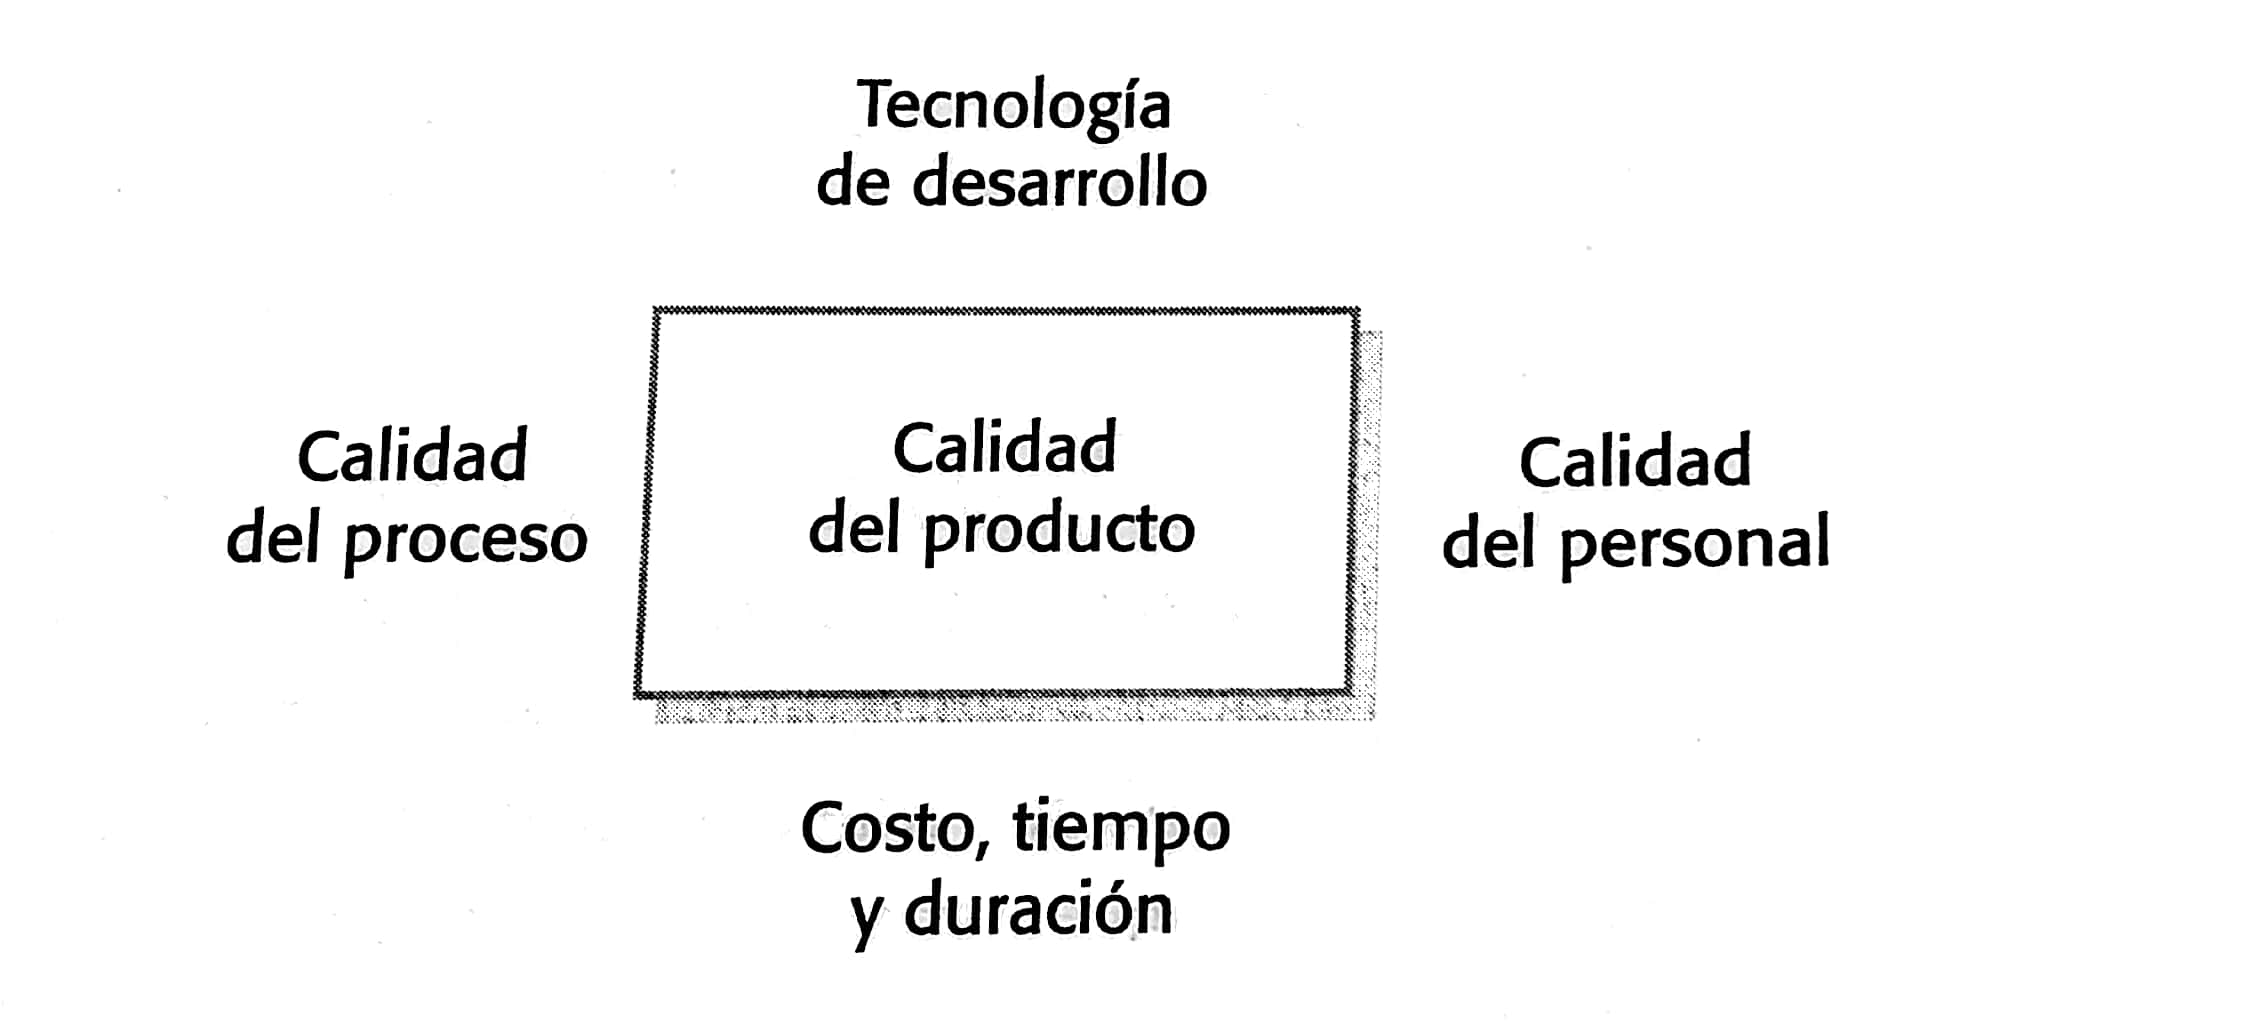
\includegraphics[scale=0.7]{M1-FactoresCalidad}
	\caption{Principales factores de calidad del producto de software\cite{sommerville_ingenierisoftware_2002}}\label{fig:M3-FactoresCalidad}
\end{figure}
\FloatBarrier

%Comentar fig 24.9 p549 relacion de metricas de proc y de prod

Para llegar a tener un software de calidad hay que tener en cuenta todos los factores mencionados anteriormente en cada una de las tres fases de la administración de la calidad: Aseguramiento, planeación y control.

La fase de control es la que se encarga de que el equipo de desarrollo cumpla los estándares y procedimientos definidos en el plan de calidad del proyecto. Esta fase puede realizarse mediante un proceso de medición.

La medición del software es un proceso en el cual se asignan valores numéricos o simbólicos a atributos de un producto o proceso software. Una métrica es una medida relacionada con un atributo de un proceso o producto software (por ejemplo). Las métricas son de control o de predicción. Las \textbf{métricas de control} se asocian al proceso de desarrollo del software (p. ej. Media de días ue se tarda en cerrar una incidencia )y las \textbf{métricas de predicción} se asocian a productos software (p. ej. Complejidad ciclomática de una función). Y ambos tipos de métricas influyen en la toma de decisiones administrativas como se observa en la figura \ref{fig:M3-MetricasProcesoYProducto}.
\begin{figure}[!h]
	\centering
	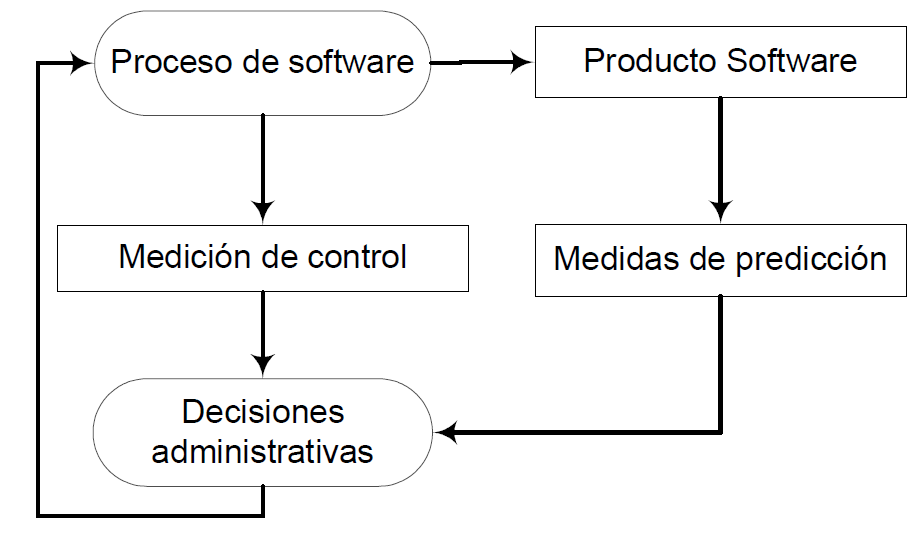
\includegraphics[scale=0.5]{M3-MetricasProcesoYProducto}
	\caption{Métricas de control y métricas de predicción\cite{sommerville_ingenierisoftware_2002}}\label{fig:M3-MetricasProcesoYProducto}
\end{figure}
%Comentar fg 24.1 p537 admin de calida en el proceso y desarrollo de software
\section{Evolución de software}
Este proyecto se centra en las métricas de control, es decir las que están asociadas al proceso de desarrollo o de evolución del software.
\subsection{Conceptos de evolución}
Una plataforma de desarrollo colaborativo como GitLab puede presentar herramientas para controlar la evolución de un proyecto software. Por ejemplo un sistema de control de versiones (VCS - \textit{Version Control System}) como Git, un sistema de seguimiento de incidencias (\textit{issue tracking system}), un sistema de integración continua (CI - \textit{Continuous Integration}), un sistema de despliegue continuo (CD - \textit{Continuous deploymen}t), etc.
Todas estas herramientas sirven para llevar un control sobre la evolución de un proyecto software ya que facilitan la comunicación entre los miembros de un equipo de desarrollo, ayudan a gestionar los cambios que producen cada uno de los miembros y proporcionan mediciones de proceso. Estas mediciones se pueden utilizar para obtener métricas de proceso que ayuden a mejorar la evolución del proyecto comparandolas con otras mediciones de otros proyectos.

\subsection{Métricas de evolución o de proceso}
Como se ha explicado antes, este proyecto trata de calcular métricas de proceso. Las métricas que se utilizan en este proyecto provienen una Master Tesis titulada \textit{sPACE: Software Project Assessment in the Course of Evolution} \cite{ratzinger_space:_2007}:\\

\textbf{\underline{I1 - Número total de issues(incidencias)}}
\begin{itemize}
	\tightlist
	\item \textbf{Categoría}: Proceso de Orientación
	\item \textbf{Descripción}: Número total de issues creadas en el repositorio
	\item \textbf{Propósito}: ¿Cuántas issues se han definido en el repositorio?
	\item \textbf{Fórmula}: NTI. NTI = número total de issues
	\item \textbf{Fuente de medición}: Proyecto en una plataforma de desarrollo colaborativo.
	\item \textbf{Interpretación}: NTI >= 0. Valores bajos indican que no se utiliza un Sistema de seguimiento de incidencias, podría ser porque el proyecto acaba de comenzar
	\item \textbf{Tipo de escala}: Absoluta
	\item \textbf{Tipo de medida}: NTI = Contador
\end{itemize}
\textbf{\underline{I2 - Commits(cambios) por issue}}
\begin{itemize}
	\tightlist
	\item \textbf{Categoría}: Proceso de Orientación
	\item \textbf{Descripción}: Número de commits por issue
	\item \textbf{Propósito}: ¿Cuál es el volumen medio de trabajo de las issues?
	\item \textbf{Fórmula}: CI = NTC/NTI. NTC = Número total de commits, NTI = Numero total de issues
	\item \textbf{Fuente de medición}: Proyecto en una plataforma de desarrollo colaborativo.
	\item \textbf{Interpretación}: CI >= 0, Si se acerca a 1 se definen bien las issues, si alto: no se definen bien las issues, si bajo: desarrollo del proyecto lento
	\item \textbf{Tipo de escala}: Ratio 
	\item \textbf{Tipo de medida}: NTC, NTI = Contador
\end{itemize}
\textbf{\underline{I3 - Porcentaje de issues cerradas}}
\begin{itemize}
	\tightlist
	\item \textbf{Categoría}: Proceso de Orientación
	\item \textbf{Descripción}: Porcentaje de issues cerradas
	\item \textbf{Propósito}: ¿Qué porcentaje de issues definidas en el repositorio se han cerrado?
	\item \textbf{Fórmula}: PIC = NTIC*100/NTI. NTIC = Número total de issues cerradas, NTI = Numero total de issues
	\item \textbf{Fuente de medición}: Proyecto en una plataforma de desarrollo colaborativo.
	\item \textbf{Interpretación}: 0 <= PIC <= 100. Cuanto más alto mejor
	\item \textbf{Tipo de escala}: Ratio
	\item \textbf{Tipo de medida}: NTI, NTIC = Contador
\end{itemize}
\textbf{\underline{TI1 - Media de días en cerrar una issue}}
\begin{itemize}
	\tightlist
	\item \textbf{Categoría}: Constantes de tiempo
	\item \textbf{Descripción}:  Media de días en cerrar una issue
	\item \textbf{Propósito}: ¿Cuánto se suele tardar en cerrar una issue? 
	\item \textbf{Fórmula}: MDCI = SUM(DCI) / NTIC . NTIC = Número total de issues cerradas, DCI = Días en cerrar la issue
	\item \textbf{Fuente de medición}: Proyecto en una plataforma de desarrollo colaborativo.
	\item \textbf{Interpretación}: MDCI >= 0. Cuanto más pequeño mejor.
	\item \textbf{Tipo de escala}: Ratio
	\item \textbf{Tipo de medida}: NTI, NTIC = Contador
\end{itemize}
\textbf{\underline{TC1 - Media de días entre commits}}
\begin{itemize}
	\tightlist
	\item \textbf{Categoría}: Constantes de tiempo
	\item \textbf{Descripción}: Media de días que pasan entre dos commits consecutivos
	\item \textbf{Propósito}: ¿Cuántos días suelen pasar desde un commit hasta el siguiente?
	\item \textbf{Fórmula}: MDEC = [Sumatorio de (TCi-TCj) desde i=1, j=0 hasta i=NTC] / NTC. NTC = Número total de commits, TC = Tiempo de Commit 
	\item \textbf{Fuente de medición}: Proyecto en una plataforma de desarrollo colaborativo.
	\item \textbf{Interpretación}: MDEC >= 0. Cuanto más pequeño mejor.
	\item \textbf{Tipo de escala}: Ratio
	\item \textbf{Tipo de medida}: NTC = Contador; TC = Tiempo
\end{itemize}
\textbf{\underline{TC2 - Días entre primer y último commit}}
\begin{itemize}
	\tightlist
	\item \textbf{Categoría}: Constantes de tiempo
	\item \textbf{Descripción}: Días transcurridos entre el primer y el ultimo commit 
	\item \textbf{Propósito}: ¿Cuantos días han pasado entre el primer y el último commit?
	\item \textbf{Fórmula}: DEPUC = TC2- TC1. DEPUC = Días entre primer y último commit, TC2 = Tiempo de último commit, TC1 = Tiempo de primer commit.
	\item \textbf{Fuente de medición}: Proyecto en una plataforma de desarrollo colaborativo.
	\item \textbf{Interpretación}: DEPUC >= 0. Mejor valores altos
	\item \textbf{Tipo de escala}: Absoluta
	\item \textbf{Tipo de medida}: TC = Tiempo
\end{itemize}
\textbf{\underline{TC3 - Ratio de actividad de commits por mes}}
\begin{itemize}
	\tightlist
	\item \textbf{Categoría}: Constantes de tiempo
	\item \textbf{Descripción}: Muestra el número de commits relativos al número de meses
	\item \textbf{Propósito}:¿Cuál es el número medio de cambios por mes?
	\item \textbf{Fórmula}: RCM = NTC / 12
	\item \textbf{Fuente de medición}: Proyecto en una plataforma de desarrollo colaborativo.
	\item \textbf{Interpretación}: RCM > 0. Cuanto más alto mejor
	\item \textbf{Tipo de escala}: Ratio
	\item \textbf{Tipo de medida}: NTC = Contador
\end{itemize}
\textbf{\underline{C1 - Número de commits en el mes pico}}
\begin{itemize}
	\tightlist
	\item \textbf{Categoría}: Constantes de tiempo
	\item \textbf{Descripción}: Número de commits en el mes que más commits se han realizado en relación con el número total de commits
	\item \textbf{Propósito}: ¿Cuál es la proporción de trabajo realizado en el mes con mayor número de cambios?
	\item \textbf{Fórmula}: CCP = NCMP / NTC. NCMP = Número de commits en el mes pico, NTC = Número total de commits
	\item \textbf{Fuente de medición}: Proyecto en una plataforma de desarrollo colaborativo.
	\item \textbf{Interpretación}: 0 <= CCP <= 1. Mejor valores intermedios
	\item \textbf{Tipo de escala}: Ratio
	\item \textbf{Tipo de medida}: NCMP, NTC = Contador
\end{itemize}

\section{Framework de medición}
Para la implementación de las métricas se ha seguido la solución basada en frameworks propuesta en \textit{Soporte de Métricas con Independencia del Lenguaje para la Inferencia de Refactorizaciones} \cite{marticorena_soporte_2005}. El framework cuyo diseño se muetra en la figura \ref{fig:MCTMotorMetricas} es independiente del lenguaje y su objetivo es la reutilización en la implementación del cálculo de métricas.
%Describir el diseño del motor de métricas, nombrar puntos de extensión
\imagen{MCTMotorMetricas}{Diagrama del Framework para el cálculo de métricas con perfiles.}
